\chapter{Лабораторная работа №4 \\
Расчёт и моделирование направленного ответвителя на связанных линиях}

Цель работы: ознакомиться с расчётом и моделированием направленного ответвителя на связанных линиях в среде Keysight Advanced Design System (ADS).

Используемое оборудование или ПО: Keysight Advanced Design System 2020 upd1.

\section{Техническое задание}

Рассчитать и спроектировать направленный ответвитель на связанных линиях на входную частоту $F_c = 7 \text{~ГГц}$, обеспечив переходное ослабление в $k = 15 \text{~дБ}$.
Провести её настройку и исследование на схемном и топологическом уровнях.

В качестве подложки использовать Arlon AD255C с относительной диэлектрической проницаемостью $\epsilon = 2.55$, тангенсом угла диэлектрических потерь $\tg{\delta} = 0.0013$, толщиной диэлектрика $H = 0.508 \text{~мм}$ и толщиной металлизации $T = 35 \text{~мкм}$.

\section{Выполнение работы}

\subsection{Создание подложки}

В первую очередь зададим параметры подложки.

Для этого в главном окне перейдём по пути Options \textrightarrow\ Technology \textrightarrow\ Edit Stackup (tech.subst) и выберем пункт Create the master substrate from scratch.
В качестве шаблона используем 25milAlumina.
Параметры подложки возьмём из технического задания.

Результат представлен на рис.~\ref{fig:directional_coupler_substrate}.

\begin{figure}
    \centering
    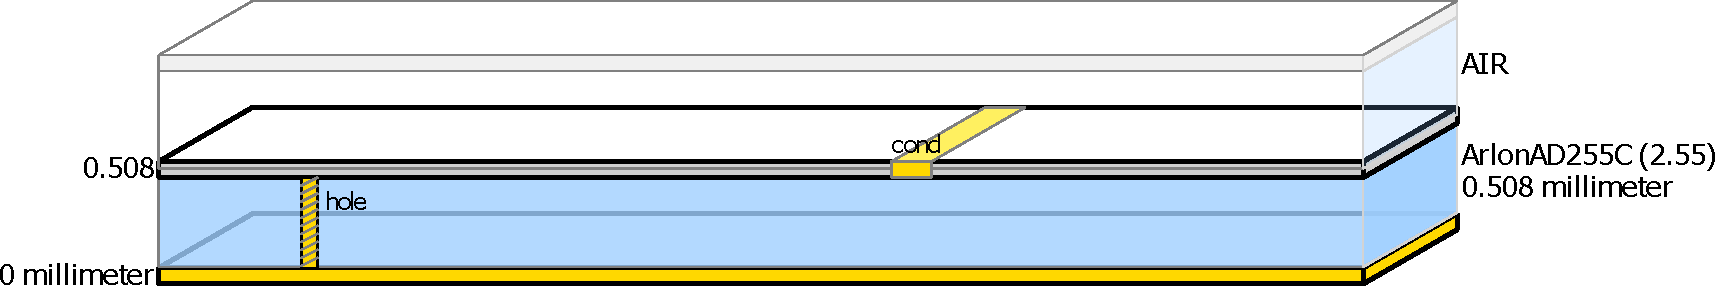
\includegraphics[width=0.9\textwidth]{directional_coupler_substrate.pdf}
    \caption{Подложка}%
    \label{fig:directional_coupler_substrate}
\end{figure}

\subsection{Модель на идеальных линиях передачи}

Соберём моделируемую схему на идеальных линиях передачи (Рис.~\ref{fig:directional_coupler_ideal_schematic}).

\begin{figure}[!ht]
    \centering
    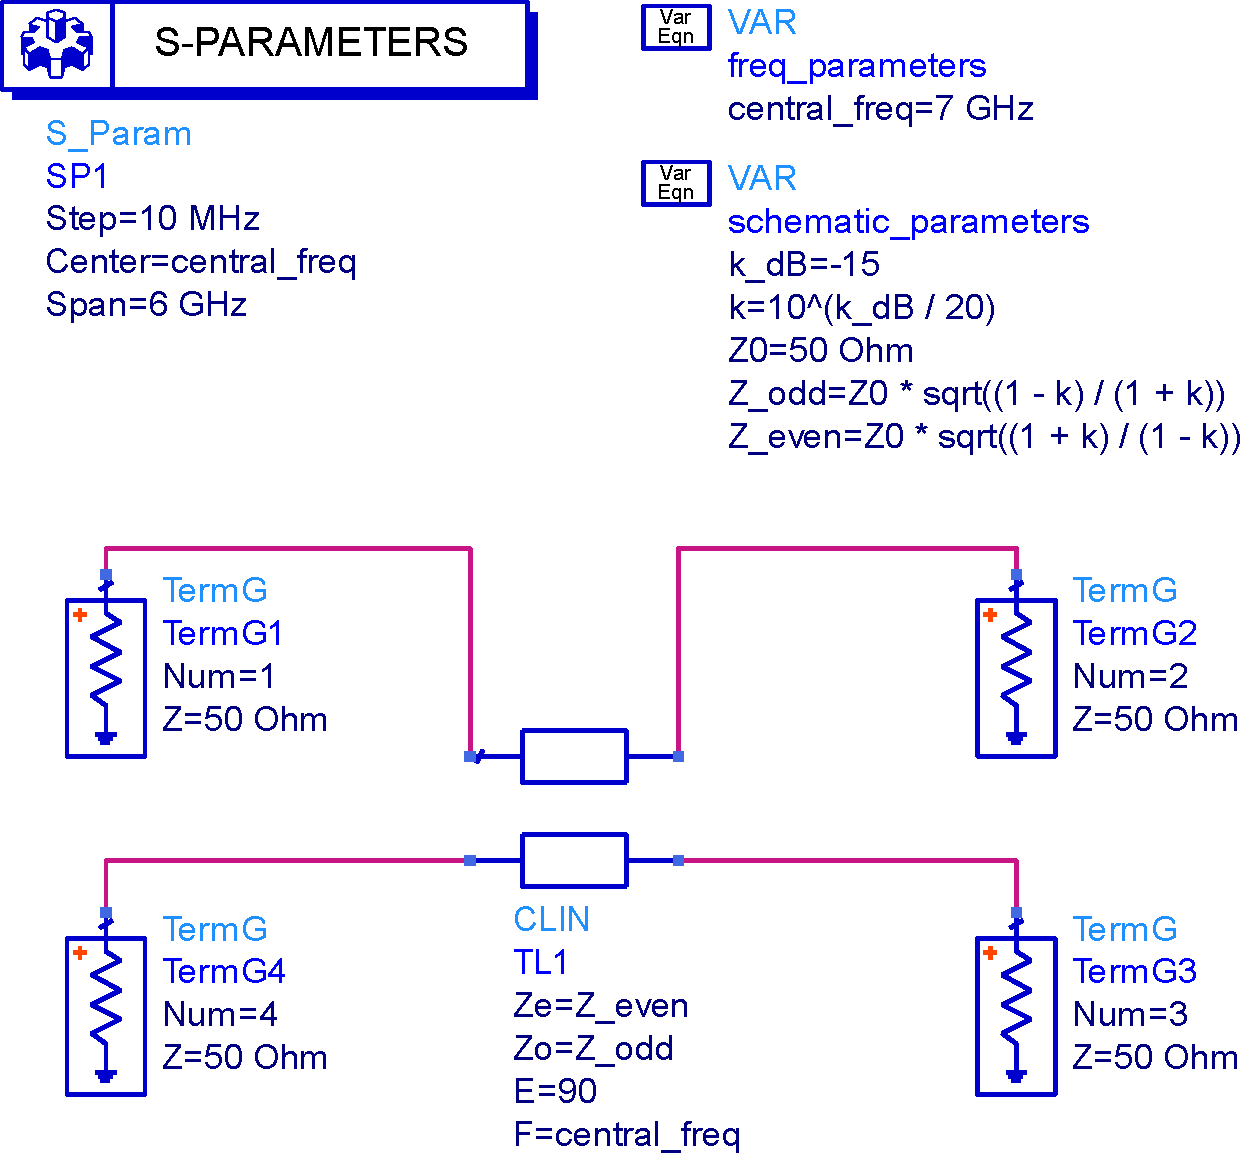
\includegraphics[width=0.6\textwidth]{directional_coupler_ideal_schematic.pdf}
    \caption{Моделируемая цепь на идеальных линиях передачи}%
    \label{fig:directional_coupler_ideal_schematic}
\end{figure}

Результаты моделирования можно увидеть на рис.~\ref{fig:directional_coupler_ideal_data_1}.

\begin{figure}[!ht]
    \centering
    \begin{subfigure}[b]{0.40\textwidth}
        \centering
        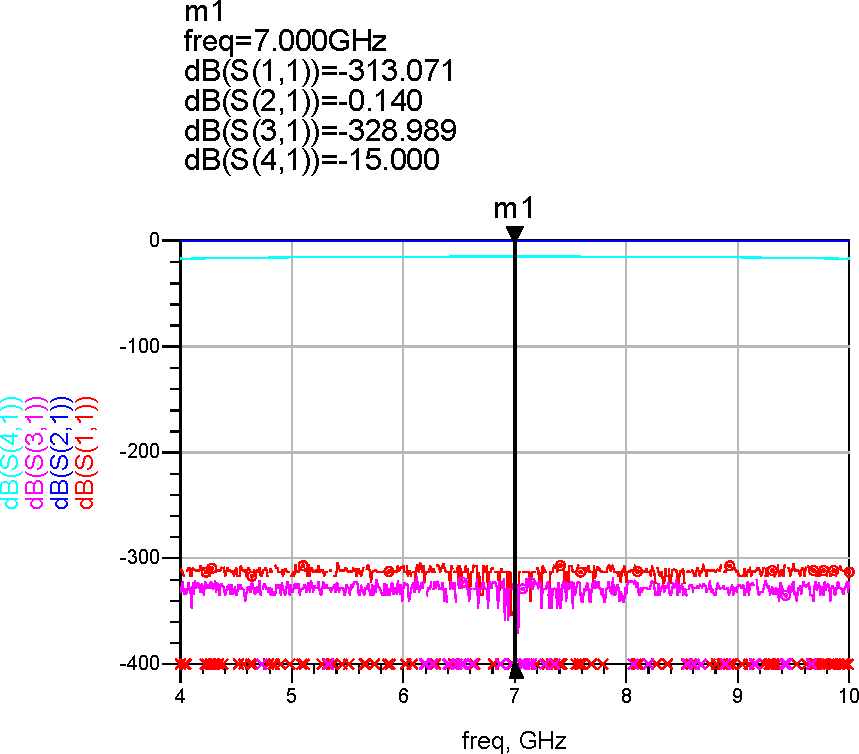
\includegraphics[width=\textwidth]{directional_coupler_ideal_data_1_freq_response.pdf}
        \caption{}%
    \label{fig:directional_coupler_ideal_data_1_freq_response}
    \end{subfigure}
    \hfill
    \begin{subfigure}[b]{0.40\textwidth}
        \centering
        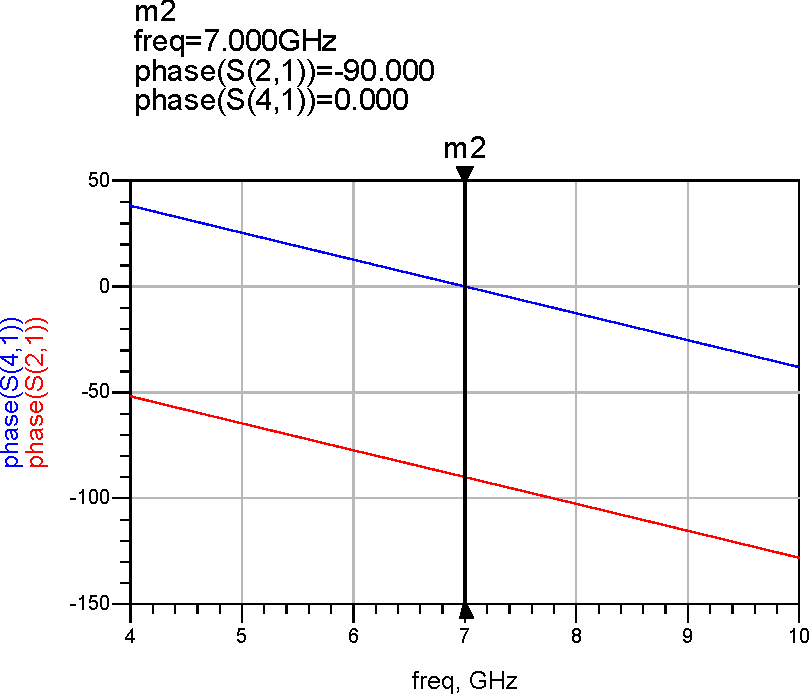
\includegraphics[width=\textwidth]{directional_coupler_ideal_data_1_phase_response.pdf}
        \caption{}%
    \label{fig:directional_coupler_ideal_data_1_phase_response}
    \end{subfigure}
    \caption{%
        (a) АЧХ моделируемой цепи;
        (б) ФЧХ моделируемой цепи
    }%
    \label{fig:directional_coupler_ideal_data_1}
\end{figure}

В этом же окне выведеи идеальную теоретическую матрицу рассеяния (Рис.~\ref{fig:directional_coupler_ideal_data_1_smatrix}).
Коэффициенты отражения $S_{11}$ и $S_{33}$, а также развязка $S_{31}$ имеют значение по амплитуде $-\infty \text{~дБ}$. Рабочие затухания $S_{21}$ и $S_{32}$ и переходные ослабления $S_{41}$ и $S_{41}$ равны $-3 \text{~дБ}$. По фазовым соотношениям видны суммарный и разностный выходы.
\begin{figure}[!ht]
    \centering
    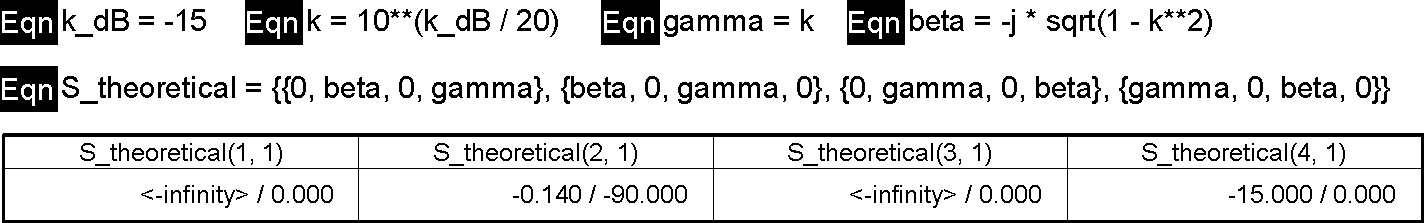
\includegraphics[width=0.8\textwidth]{directional_coupler_ideal_data_1_smatrix}
    \caption{Идеальная теоретическая матрица рассеяния}%
    \label{fig:directional_coupler_ideal_data_1_smatrix}
\end{figure}

\subsection{Модель на схемном уровне в микрополосковом исполнении}

Для расчёта геометрических размеров нескольких видов линий передач воспользуемся инструментом LineCalc, которую можно найти по пути Tools \textrightarrow\ LineCalc \textrightarrow\ Start LineCalc.

В подокне Substrate Parameters задаём параметры подложки из технического задания, в подокне Component Parameters задаём частоту из технического задания, а в подокне Electrical --- импеданс и электрическую длину, для которых ведётся расчёт.
После этого, нажав кнопку Synthesize, получим в подокне Physical искомые геометрические размеры.

Расчитаем таким образом необходимые геометрические размеры отрезков.
Получим $W_{coupled} = 1.293 \text{~мм}$ и $S_{coupled} = 0.324 \text{~мм}$, $L_\text{coupled} = 7.450 \text{~мм}$, а $W_{50} = 1.382 \text{~мм}$.

Построим дополнительную схему для подбора оптимального значения среза $M$ (Рис.~\ref{fig:directional_coupler_MLIN_schematic_1}). Запустим моделирование и построим зависимость $dB(S_{11})$ от частоты (Рис.~\ref{fig:directional_coupler_MLIN_data_display_1}) и выберем значение $M$, соответствующее линии, которая лежит ниже остальных.

\begin{figure}[!ht]
    \centering
    \begin{subfigure}[b]{0.50\textwidth}
        \centering
        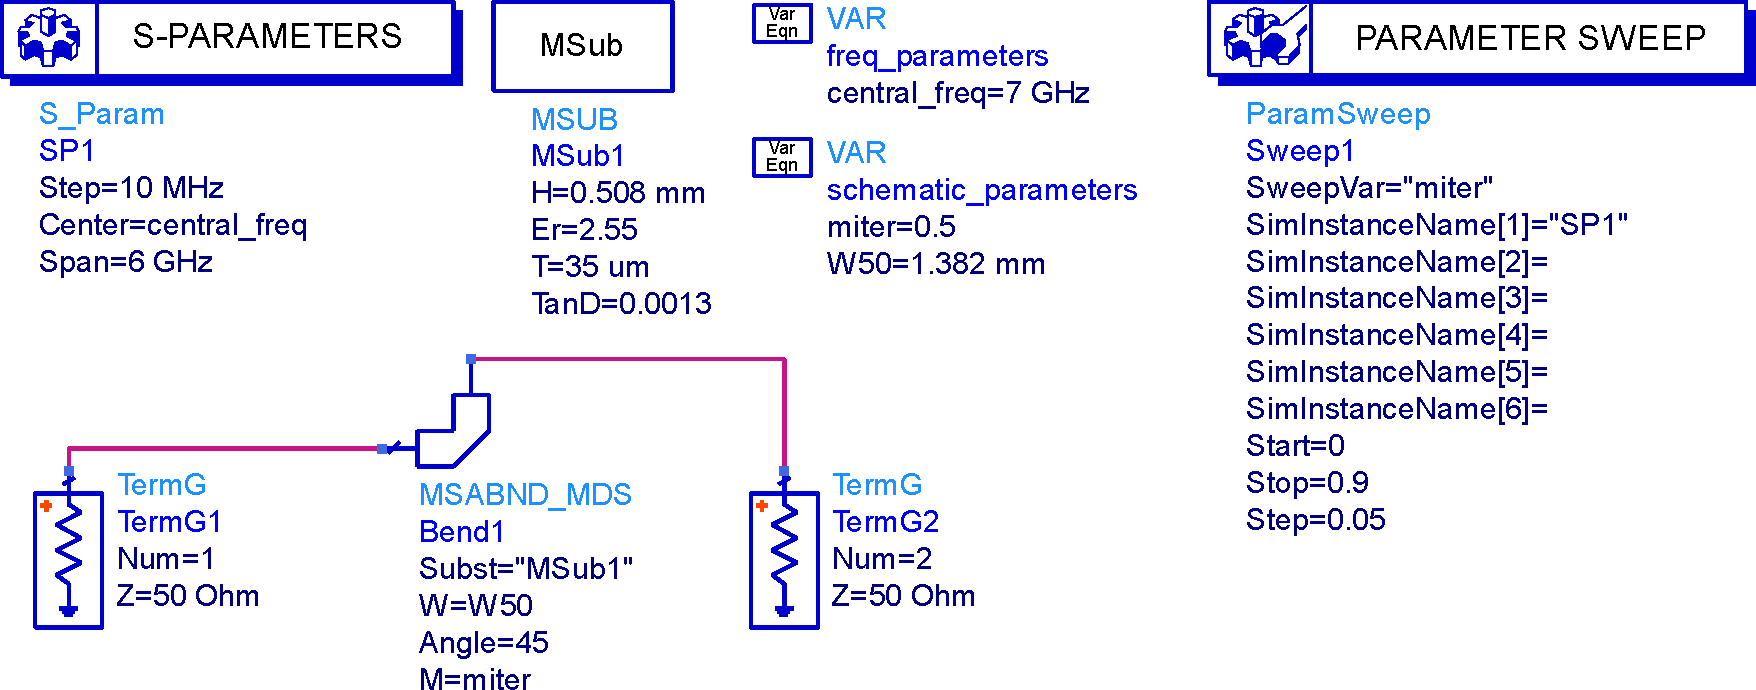
\includegraphics[width=\textwidth]{directional_coupler_MLIN_schematic_1.pdf}
        \caption{}%
    \label{fig:directional_coupler_MLIN_schematic_1}
    \end{subfigure}
    \hfill
    \begin{subfigure}[b]{0.40\textwidth}
        \centering
        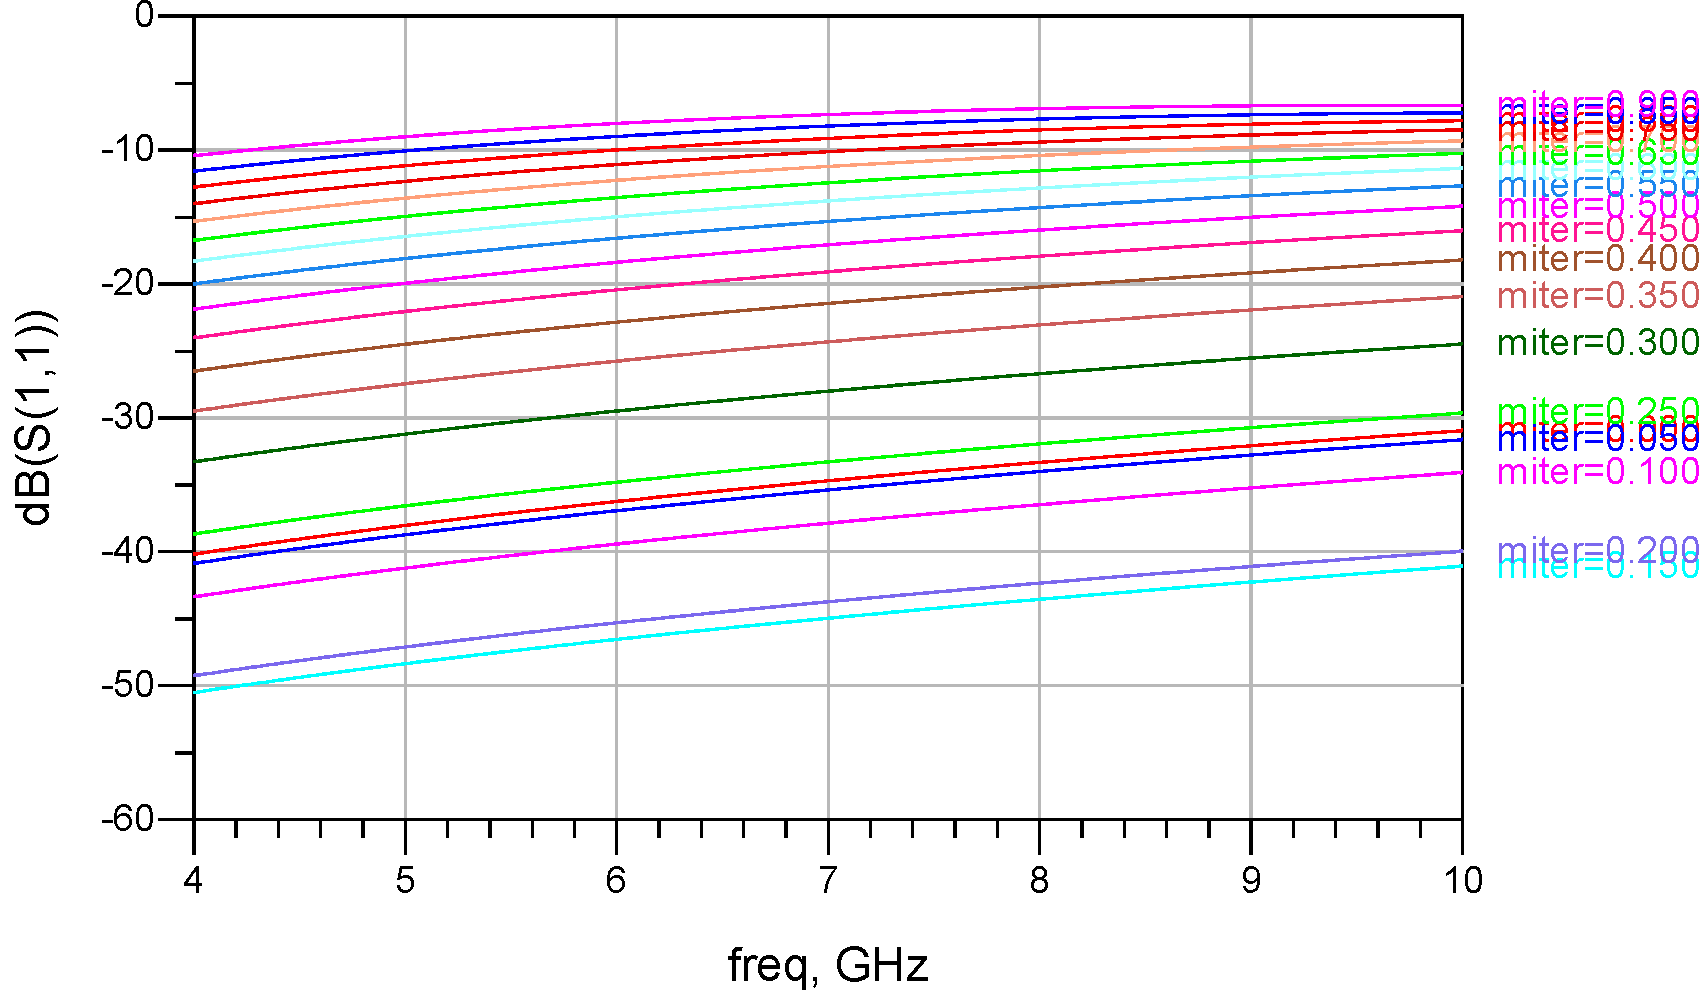
\includegraphics[width=\textwidth]{directional_coupler_MLIN_data_display_1.pdf}
        \caption{}%
    \label{fig:directional_coupler_MLIN_data_display_1}
    \end{subfigure}
    \caption{%
        (а) Схема для подбора значения среза $M$;
        (б) моделирование
    }%
    \label{fig:directional_coupler_MLIN_miter}
\end{figure}

Построим моделируемую схему в микрополосковом исполнении (Рис.~\ref{fig:directional_coupler_MLIN_schematic_2}), после чего запустим расчёт и выведем АЧХ (Рис.~\ref{fig:directional_coupler_MLIN_data_1_responses}).

\begin{figure}[!ht]
    \centering
    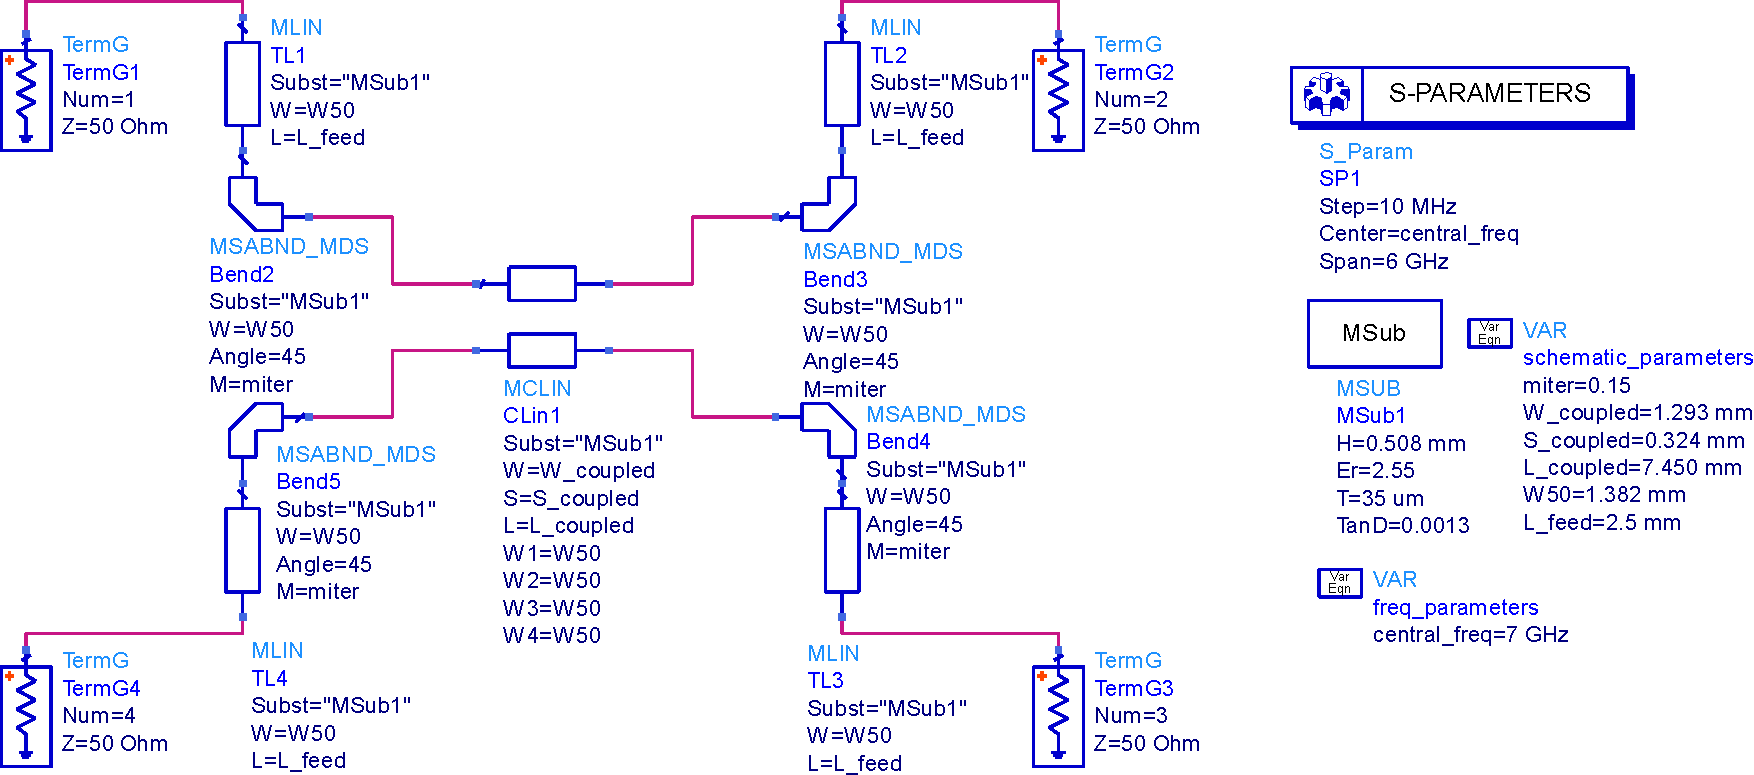
\includegraphics[width=0.8\textwidth]{directional_coupler_MLIN_schematic_2.pdf}
    \caption{Моделируемая схема в микрополосковом исполнении}%
    \label{fig:directional_coupler_MLIN_schematic_2}
\end{figure}

\begin{figure}[!ht]
    \begin{subfigure}[b]{0.45\textwidth}
        \centering
        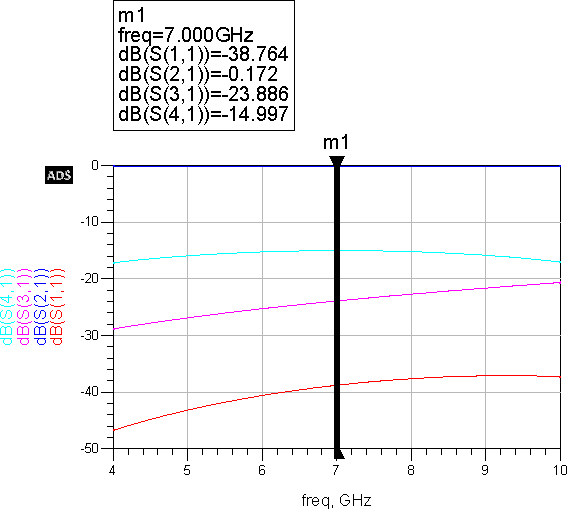
\includegraphics[width=\textwidth]{directional_coupler_MLIN_data_1_freq_response.pdf}
        \caption{}%
    \label{fig:directional_coupler_MLIN_data_1_freq_response}
    \end{subfigure}
    \hfill
    \begin{subfigure}[b]{0.45\textwidth}
        \centering
        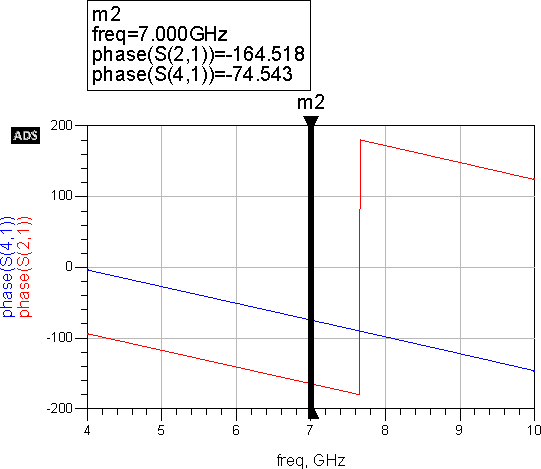
\includegraphics[width=\textwidth]{directional_coupler_MLIN_data_1_phase_response.pdf}
        \caption{}%
    \label{fig:directional_coupler_MLIN_data_1_phase_response}
    \end{subfigure}
    \caption{%
        Результаты моделирования схемы:
        (а) АЧХ;
        (б) ФЧХ
    }%
    \label{fig:directional_coupler_MLIN_data_1_responses}
\end{figure}

Из выведенных соотношений можно сделать следующие выводы:
\begin{itemize}
    \item согласование по входу $dB(S_{11})$ осталось хорошим ($\approx -40 \text{~дБ}$);
    \item рабочее затухание $dB(S_{21})$ в пределах $-0.2 \text{~дБ}$;
    \item переходное ослабление $dB(S_{41})$ близко требуемому значениею $k = -15 \text{~дБ}$;
    \item развязка $dB(S_{31})$ приняла
\end{itemize}

Неравномерность частотных характеристик в заданном диапазоне можно увидеть на рис.~\ref{fig:directional_coupler_MLIN_data_2_ripple_freq_response}.

\begin{figure}[!ht]
    \centering
    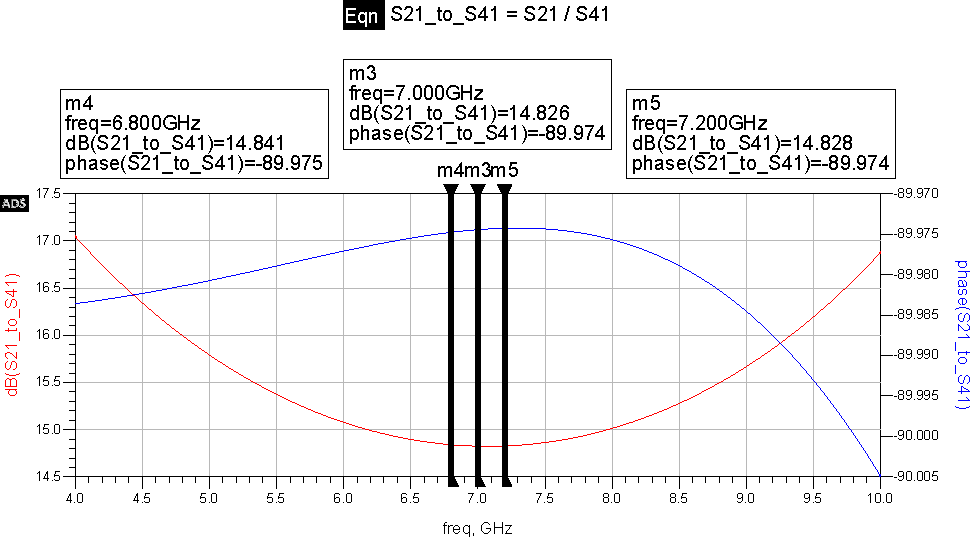
\includegraphics[width=0.8\textwidth]{directional_coupler_MLIN_data_1_ripple_freq_response.pdf}
    \caption{Неравномерность рабочего затухания и переходного ослабления}%
    \label{fig:directional_coupler_MLIN_data_1_ripple_freq_response}
\end{figure}

\subsection{Модель на топологическом уровне}

Скопируем схему в микрополосковом исполнении в новую ячейку. Сделаем её двухуровневой, перенеся во внутренний уровень все полосковые устройства. Сделать это можно по команде Edit \textrightarrow\ Component \textrightarrow\ Create Hierarchy.

В результате получим схему верхнего уровня (Рис.~\ref{fig:directional_coupler_EM_schematic_1}) и схему нижнего уровня (Рис.~\ref{fig:directional_coupler_EM_inner_schematic}).

\begin{figure}[!ht]
    \centering
    \begin{subfigure}[b]{0.55\textwidth}
        \centering
        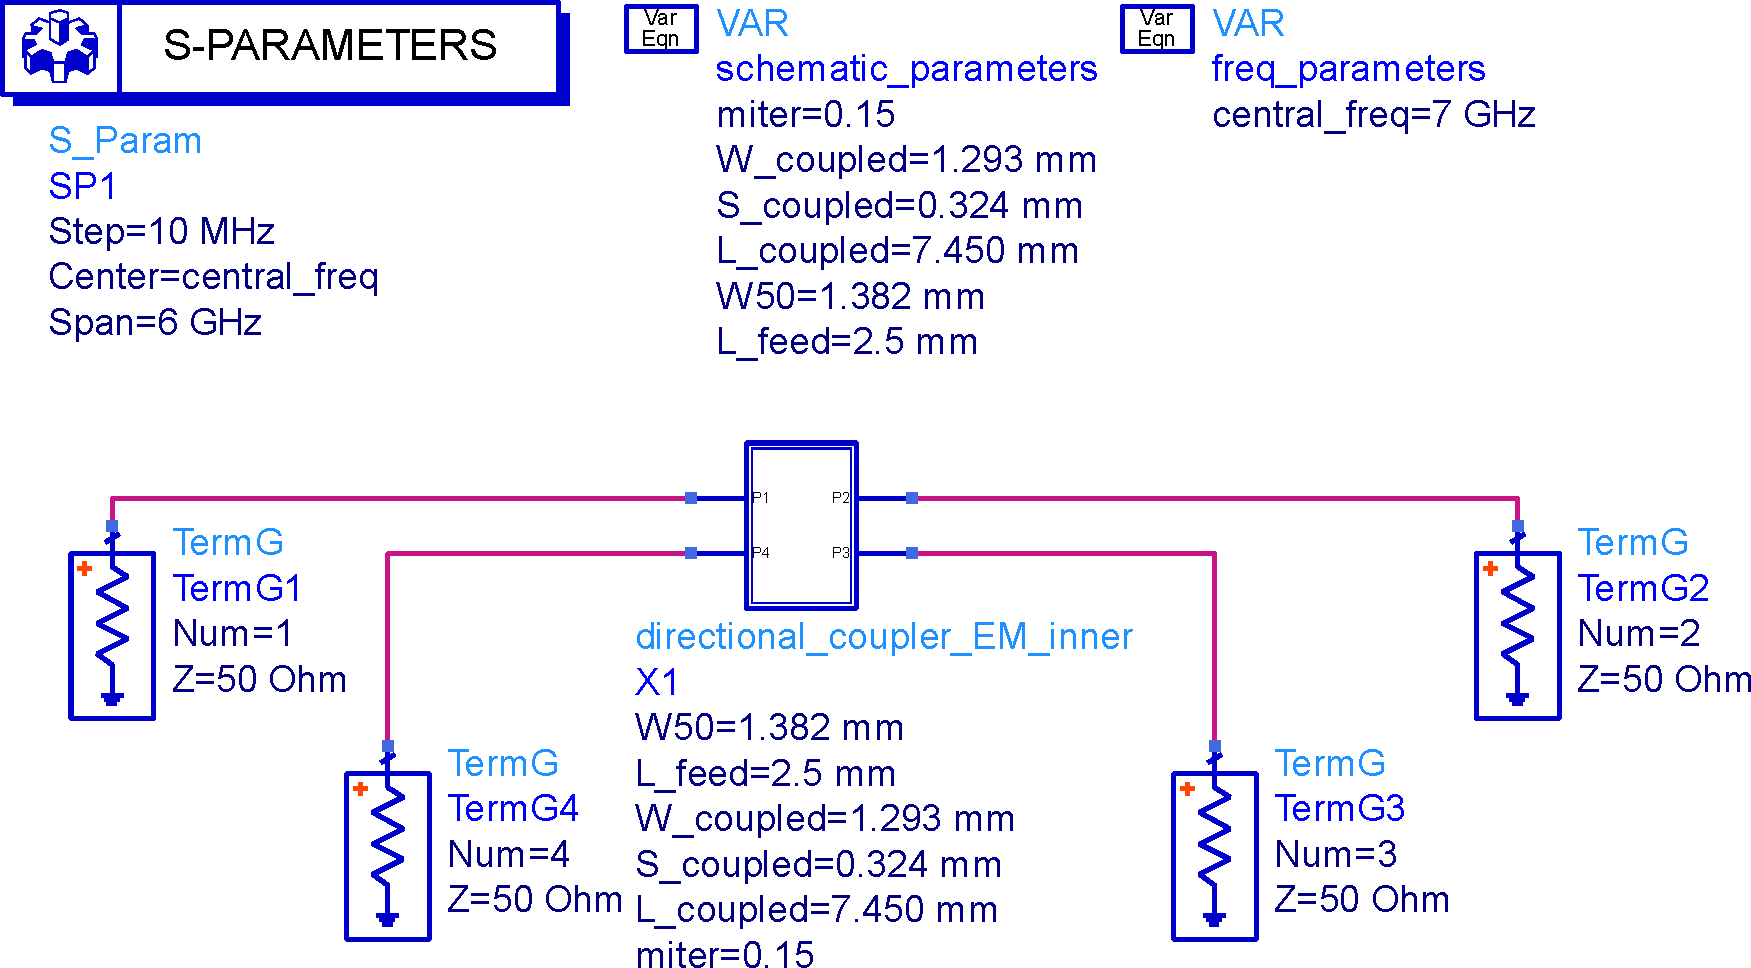
\includegraphics[width=\textwidth]{directional_coupler_EM_schematic_1.pdf}
        \caption{}%
    \label{fig:directional_coupler_EM_schematic_1}
    \end{subfigure}
    \hfill
    \begin{subfigure}[b]{0.35\textwidth}
        \centering
        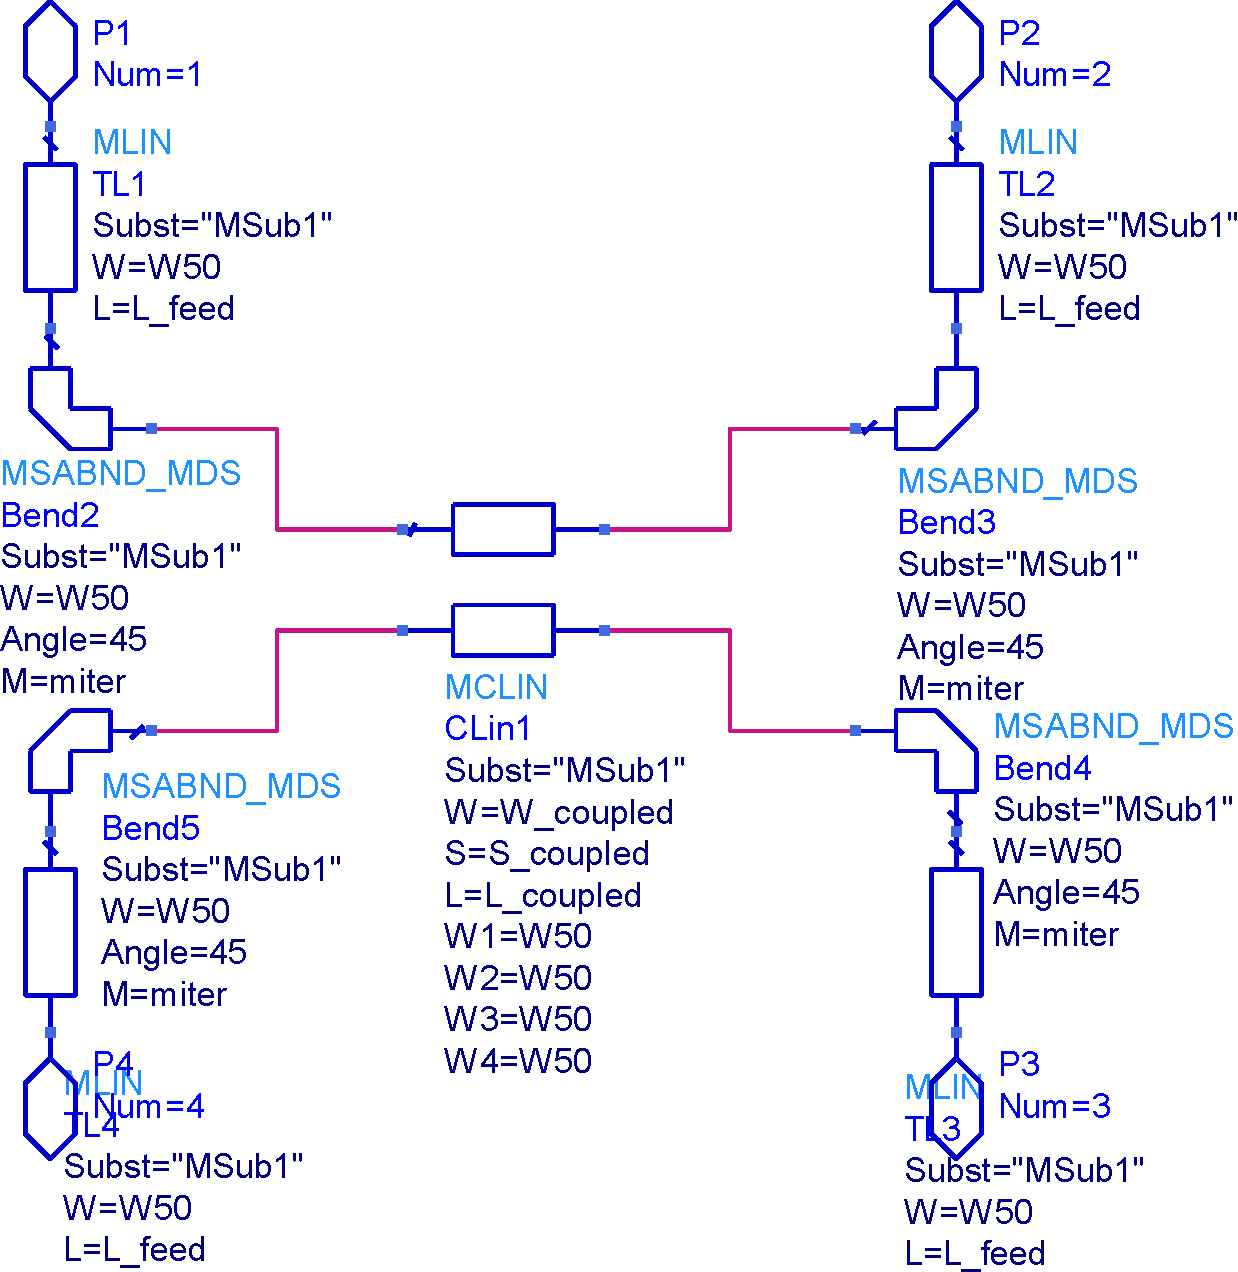
\includegraphics[width=\textwidth]{directional_coupler_EM_inner_schematic.pdf}
        \caption{}%
    \label{fig:directional_coupler_EM_inner_schematic}
    \end{subfigure}
    \caption{%
        Моделируемая схема на топологическом уровне:
        (a) внешнаяя схема;
        (б) внутренняя схема
    }%
    \label{fig:directional_coupler_EM_schematics}
\end{figure}

Перейдём в схему нижнего уровня. Для получения топологического представления воспользуемся функцией Layout \textrightarrow\ Generate/Update Layout.

\begin{comment}
Топологическое представление создано верно (Рис.~\ref{fig:directional_coupler_layout_check}).

\begin{wrapfigure}{l}{0.4\textwidth}
    \centering
    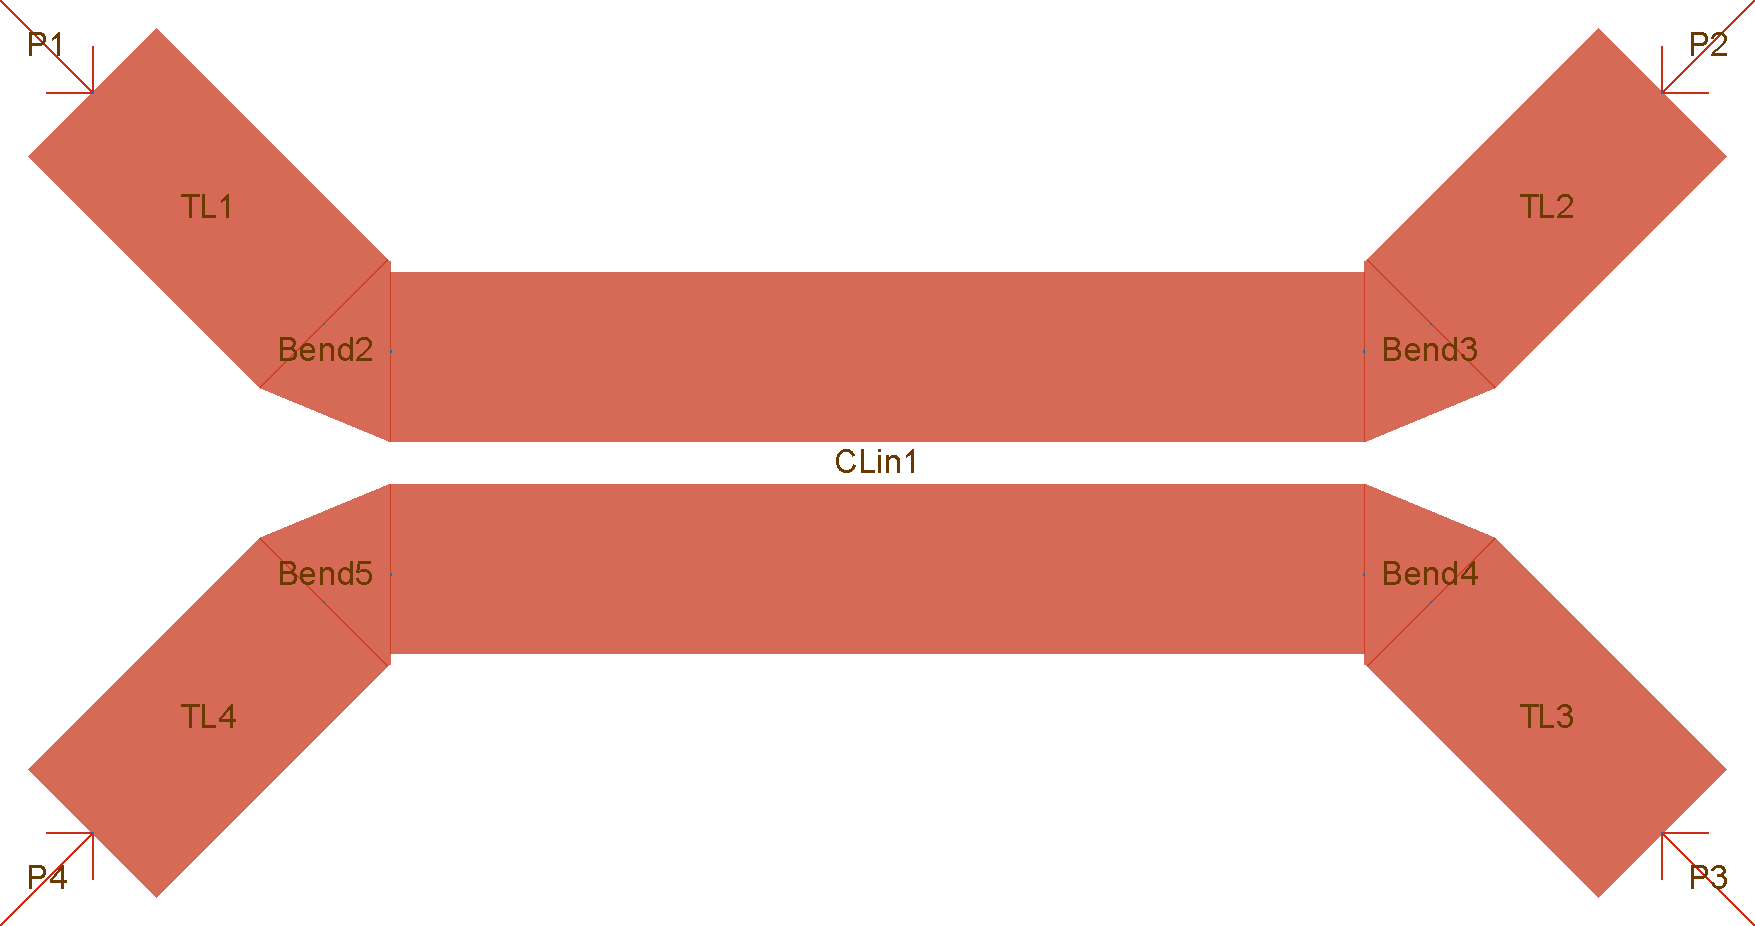
\includegraphics[width=0.4\textwidth]{directional_coupler_layout_check.pdf}
    \caption{Проверка топологического представления}%
    \label{fig:directional_coupler_layout_check}
\end{wrapfigure}
\end{comment}

\begin{wrapfigure}{r}{0.4\textwidth}
    \centering
    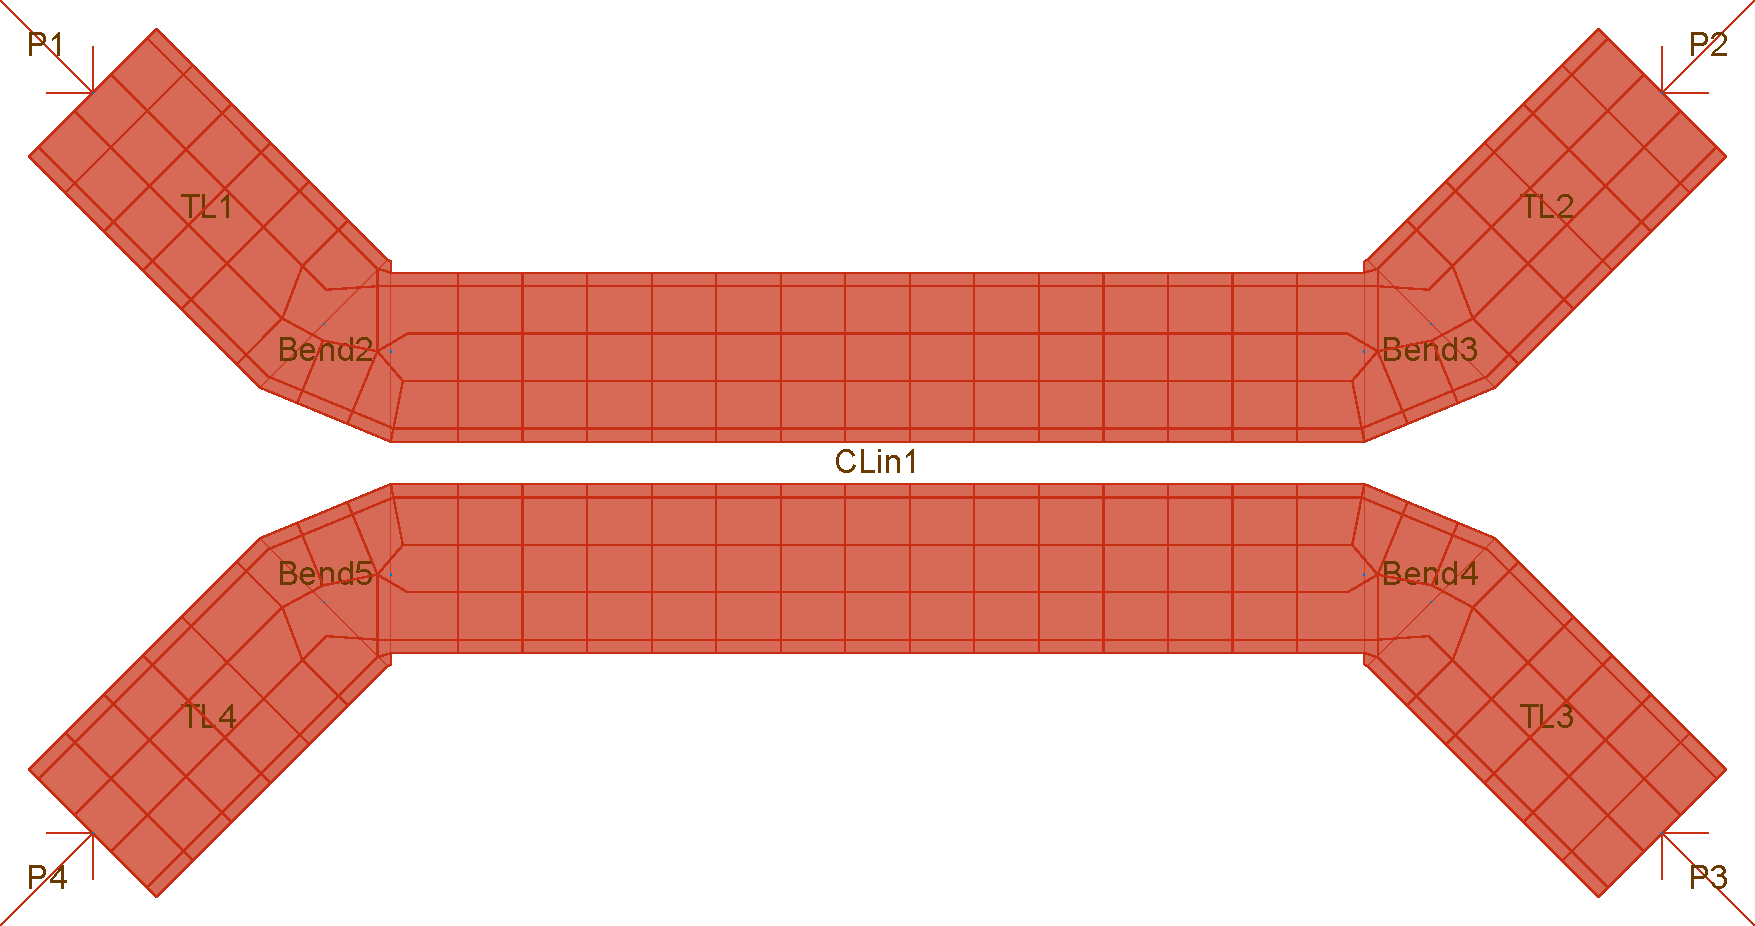
\includegraphics[width=0.4\textwidth]{directional_coupler_layout_sparam.pdf}
    \caption{Сетка на топологическом представлении после проведения EM-моделирования}%
    \label{fig:directional_coupler_layout_sparam}
\end{wrapfigure}
Перейдём в окно File \textrightarrow\ Customize Pcell.
Сделаем схему параметризуемой, выбрав в выпадающем списке тип Parameterized sub network Pcell.
Также убедимся в том, что выставлены галочки напротив Support non-90 degree rotation и Support unit and database resolution for ADS 2015 and older.

В окне File \textrightarrow\ Cell Parameters определим параметры $W_{50}$, $L_\text{feed}$, $L_\text{shunt}$, $L_\text{serial}$.

Для EM-моделирования создадим сущность emSetup.
Это можно сделать в окне EM \textrightarrow\ Simulation Setting.
Определим параметры в соответствии с требованиями.

Запустим EM-моделирование нажатием кнопки Simulate.
В результате на топологии появится сетка (Рис.~\ref{fig:directional_coupler_layout_sparam}).

Из окна emSetup можно обновить отображение элемента на схеме.
Сделаем так, чтоб оно подгружалось из топологии.
В итоге схема приобретёт вид как на рис.~\ref{fig:directional_coupler_EM_schematic_2}.

\begin{figure}[!ht]
    \centering
    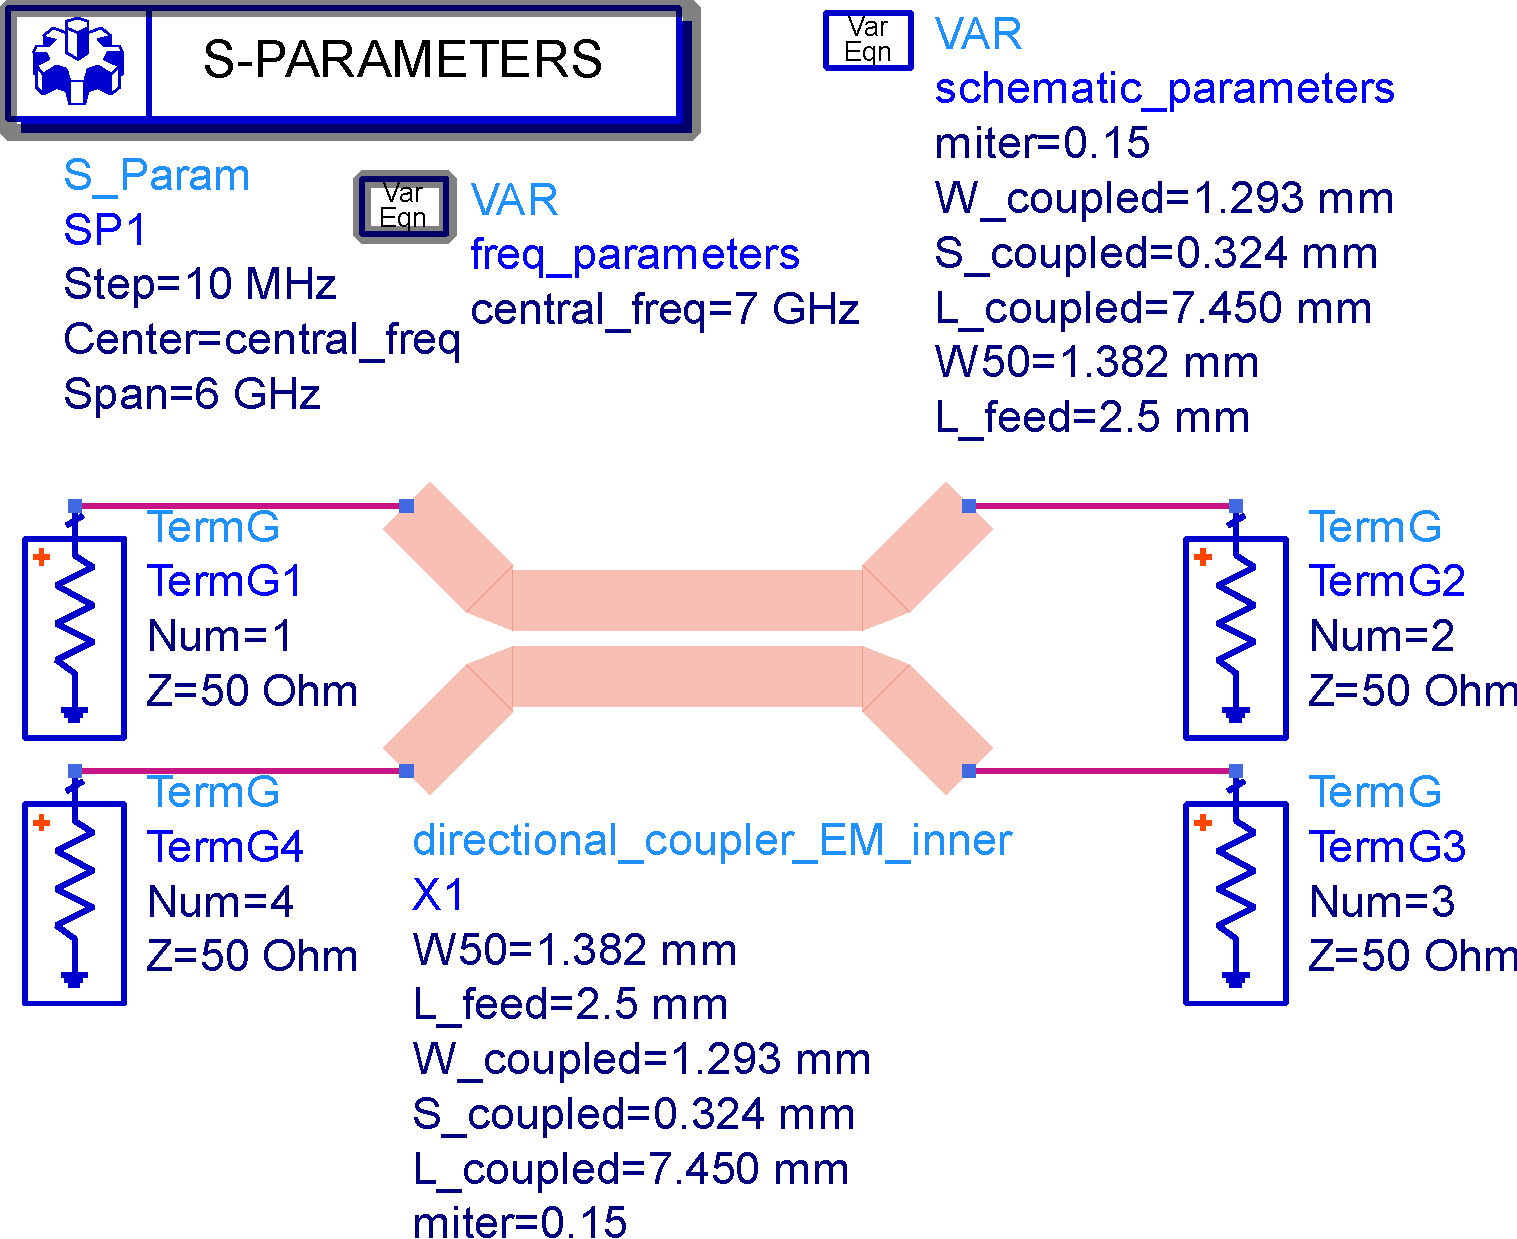
\includegraphics[width=0.6\textwidth]{directional_coupler_EM_schematic_2.pdf}
    \caption{Итоговый вид схемы}%
    \label{fig:directional_coupler_EM_schematic_2}
\end{figure}

Запустим моделирование и отобразим частотные характеристики (Рис.~\ref{fig:directional_coupler_EM_data_1_freq_response}) и неравномерность характеристик (Рис.~\ref{fig:directional_coupler_EM_data_1_ripple_response}).

\begin{figure}[!ht]
    \begin{subfigure}[b]{0.45\textwidth}
        \centering
        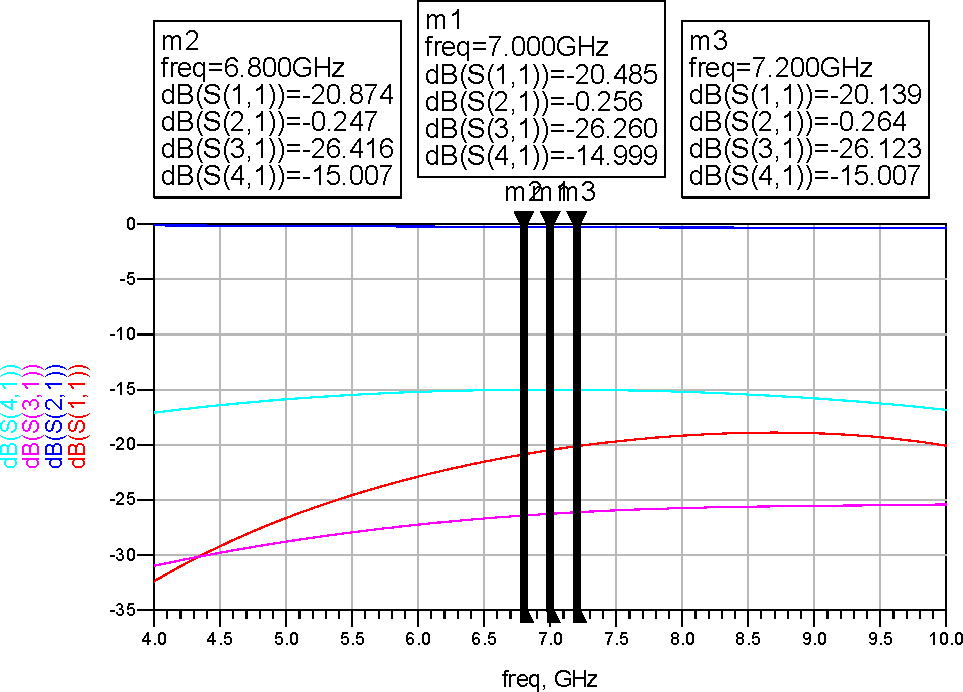
\includegraphics[width=\textwidth]{directional_coupler_EM_data_1_freq_response.pdf}
        \caption{}%
        \label{fig:directional_coupler_EM_data_1_freq_response}
    \end{subfigure}
    \hfill
    \begin{subfigure}[b]{0.45\textwidth}
        \centering
        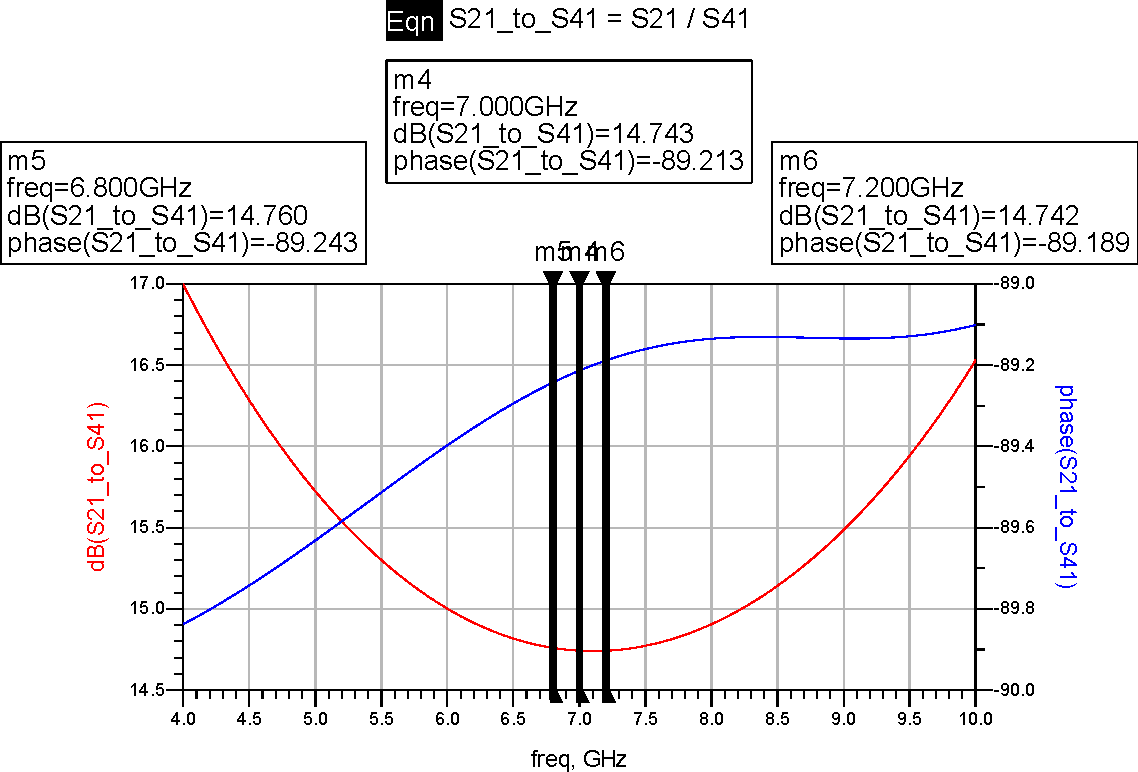
\includegraphics[width=\textwidth]{directional_coupler_EM_data_1_ripple_response.pdf}
        \caption{}%
        \label{fig:directional_coupler_EM_data_1_ripple_response}
    \end{subfigure}
    \caption{%
        (а) АЧХ моделируемой схемы в топологическом представлении;
        (б) неравномерность характеристик моделируемой схемы в топологическом представлении
    }%
    \label{fig:directional_coupler_EM_data_1}
\end{figure}
